\documentclass[12pt,a4paper,landscape]{article}

% ============================================================
% PACKAGES
% ============================================================
\usepackage[utf8]{inputenc}
\usepackage[T1]{fontenc}
\usepackage{graphicx}
\usepackage{xcolor}
\usepackage{geometry}
\usepackage{tikz}
\usepackage{array}
\usepackage{enumitem}
\usepackage{ragged2e}
\usepackage{helvet}
\usepackage{fancyhdr}
\usepackage{colortbl}
\usepackage{eso-pic}
\usepackage{microtype}

\usetikzlibrary{arrows.meta}

% ============================================================
% PAGE SETUP
% ============================================================
\geometry{
    a4paper,
    landscape,
    left=1.25cm,
    right=1.25cm,
    top=0.95cm,
    bottom=0.85cm,
    headheight=15pt,
    headsep=0.25cm,
    footskip=15pt
}

\setlength{\headheight}{15pt}
\setlength{\footskip}{15pt}

\renewcommand{\familydefault}{\sfdefault}

% ============================================================
% COLORS
% ============================================================
\definecolor{DarkBlue}{RGB}{25,65,125}
\definecolor{Red}{RGB}{220,45,45}
\definecolor{LightGray}{RGB}{245,245,245}
\definecolor{BorderGray}{RGB}{190,190,190}
\definecolor{DarkGray}{RGB}{55,55,55}
\definecolor{White}{RGB}{255,255,255}

% ============================================================
% HEADER / FOOTER
% ============================================================
\pagestyle{fancy}
\fancyhf{}

\fancyhead[L]{
    \textcolor{DarkBlue}{
        \small\bfseries
        Department of Computer Science, University of Sindh
    }
}

\fancyhead[R]{
    \textcolor{DarkGray}{
        \small Mini Assignment -- HCI \& Computer Graphics
    }
}

\fancyfoot[C]{
    \textcolor{DarkGray}{\small\thepage}
}

\renewcommand{\headrulewidth}{0.5pt}
\renewcommand{\footrulewidth}{0.25pt}

% ============================================================
% PAGE TITLE
% ============================================================
\newcommand{\pagetitle}[1]{

    \begin{center}

        {\color{DarkBlue}
        \fontsize{21}{24}\selectfont
        \bfseries #1}

        \vspace{0.15cm}

        \rule{18.5cm}{0.5pt}

    \end{center}

    \vspace{0.30cm}
}

% ============================================================
% DOCUMENT
% ============================================================
\begin{document}


% ============================================================
% PAGE 1 -- COVER PAGE
% ============================================================

\thispagestyle{empty}

\begin{tikzpicture}[remember picture,overlay]

\node[
    anchor=center,
    inner sep=0pt
]
at (current page.center)
{
    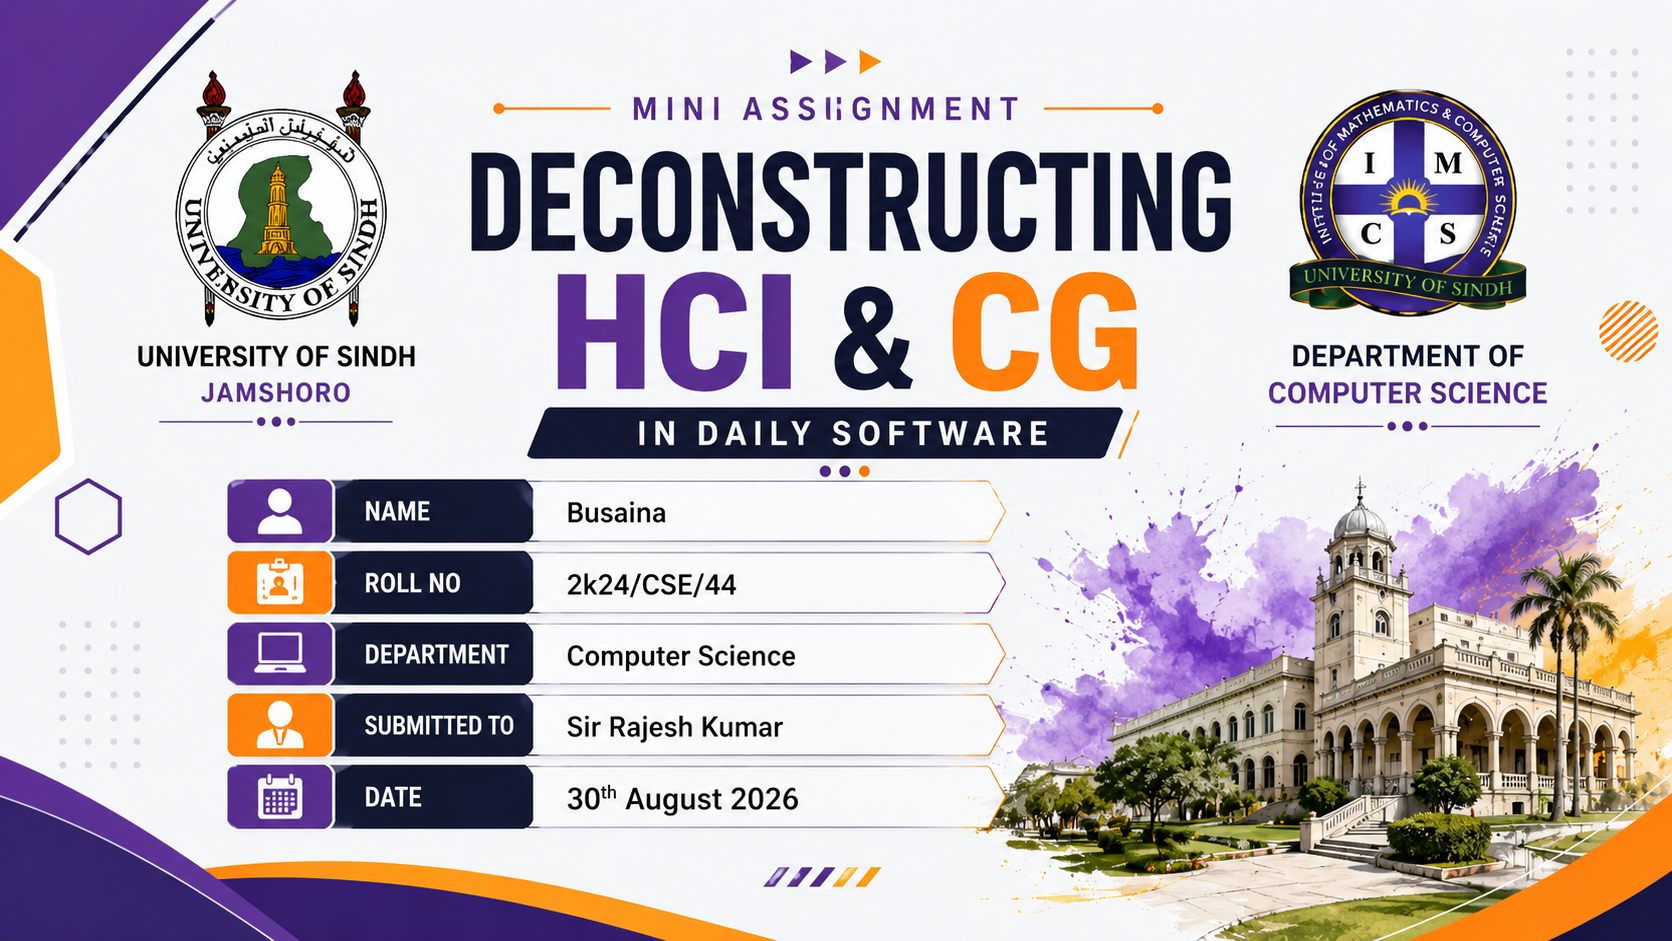
\includegraphics[
        width=\paperwidth,
        height=\paperheight
    ]{CoverPage.png}
};

\end{tikzpicture}

\clearpage


% ============================================================
% PAGE 2 -- HCI FOCUS
% ============================================================

\pagestyle{fancy}

\pagetitle{SCREENSHOT 1: HCI FOCUS}

% ============================================================
% HCI SCREENSHOT
% ============================================================

\begin{center}

\begin{tikzpicture}

% ------------------------------------------------------------
% HCI IMAGE
% ------------------------------------------------------------

\node[
    inner sep=0pt,
    anchor=north west
] (hci) at (0,0)
{
    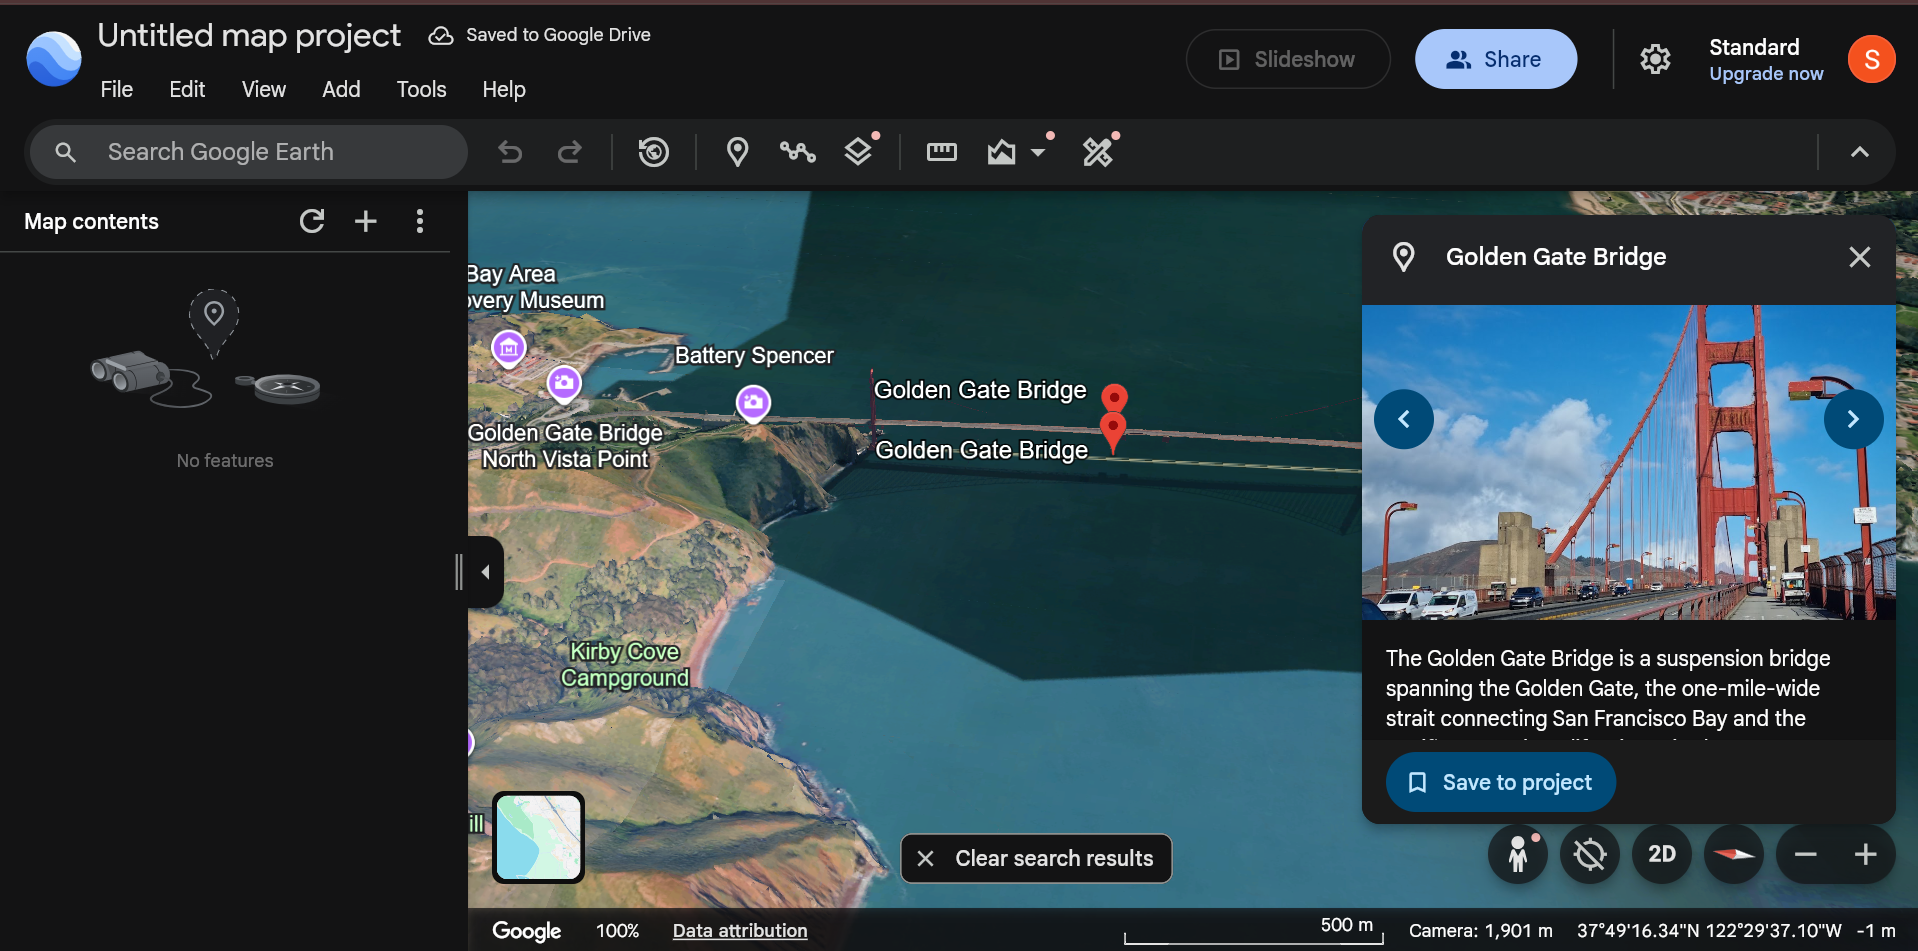
\includegraphics[
        width=18.7cm
    ]{hci_golden_gate.png}
};


% ============================================================
% HCI ANNOTATION 1 -- SEARCH BAR
% ============================================================

\node[
    circle,
    fill=Red,
    draw=White,
    line width=1.2pt,
    minimum size=0.60cm,
    inner sep=0pt,
    text=White,
    font=\bfseries\large
]
at ([xshift=2.0cm,yshift=-0.75cm]hci.north west)
{1};

\draw[
    -{Latex[length=3mm]},
    line width=1.5pt,
    Red
]
([xshift=2.0cm,yshift=-1.05cm]hci.north west)
--
([xshift=2.65cm,yshift=-1.10cm]hci.north west);


% ============================================================
% HCI ANNOTATION 2 -- NAVIGATION CONTROLS
% ============================================================

\node[
    circle,
    fill=Red,
    draw=White,
    line width=1.2pt,
    minimum size=0.60cm,
    inner sep=0pt,
    text=White,
    font=\bfseries\large
]
at ([xshift=17.0cm,yshift=-7.85cm]hci.north west)
{2};

\draw[
    -{Latex[length=3mm]},
    line width=1.5pt,
    Red
]
([xshift=16.72cm,yshift=-7.70cm]hci.north west)
--
([xshift=15.55cm,yshift=-7.45cm]hci.north west);


% ============================================================
% HCI ANNOTATION 3 -- INFORMATION PANEL
% ============================================================

\node[
    circle,
    fill=Red,
    draw=White,
    line width=1.2pt,
    minimum size=0.60cm,
    inner sep=0pt,
    text=White,
    font=\bfseries\large
]
at ([xshift=15.35cm,yshift=-2.15cm]hci.north west)
{3};

\draw[
    -{Latex[length=3mm]},
    line width=1.5pt,
    Red
]
([xshift=15.12cm,yshift=-2.35cm]hci.north west)
--
([xshift=14.05cm,yshift=-2.75cm]hci.north west);

\end{tikzpicture}

\end{center}


% ============================================================
% HCI EXPLANATIONS
% ============================================================

\vspace{0.22cm}

\begin{enumerate}[
    label=\textcolor{Red}{\bfseries\arabic*.},
    leftmargin=0.72cm,
    rightmargin=0.25cm,
    itemsep=3pt,
    topsep=0pt,
    parsep=0pt
]

\item
\textbf{Search Bar (Top-Left):}
Allows users to quickly search for any location worldwide.
The search function provides a direct way to enter a destination
and locate it on the map, reducing the effort required to find
places.

\item
\textbf{3D Navigation Controls (Bottom-Right):}
Includes zoom, rotation, compass, and view controls that let
users explore the 3D environment from different angles.
These controls provide clear visual affordances for manipulating
the map view.

\item
\textbf{Information Panel (Right-Side):}
Displays information about the selected location, including
its name, image, description, and the option to save the place
to the project. This provides immediate contextual feedback
after selecting a landmark.

\end{enumerate}


% ============================================================
% PAGE BREAK
% ============================================================

\newpage


% ============================================================
% PAGE 3 -- CG FOCUS
% ============================================================

\pagetitle{SCREENSHOT 2: CG FOCUS}

% ============================================================
% CG SCREENSHOT
% ============================================================

\begin{center}

\begin{tikzpicture}

% ------------------------------------------------------------
% CG IMAGE
% ------------------------------------------------------------

\node[
    inner sep=0pt,
    anchor=north west
] (cg) at (0,0)
{
    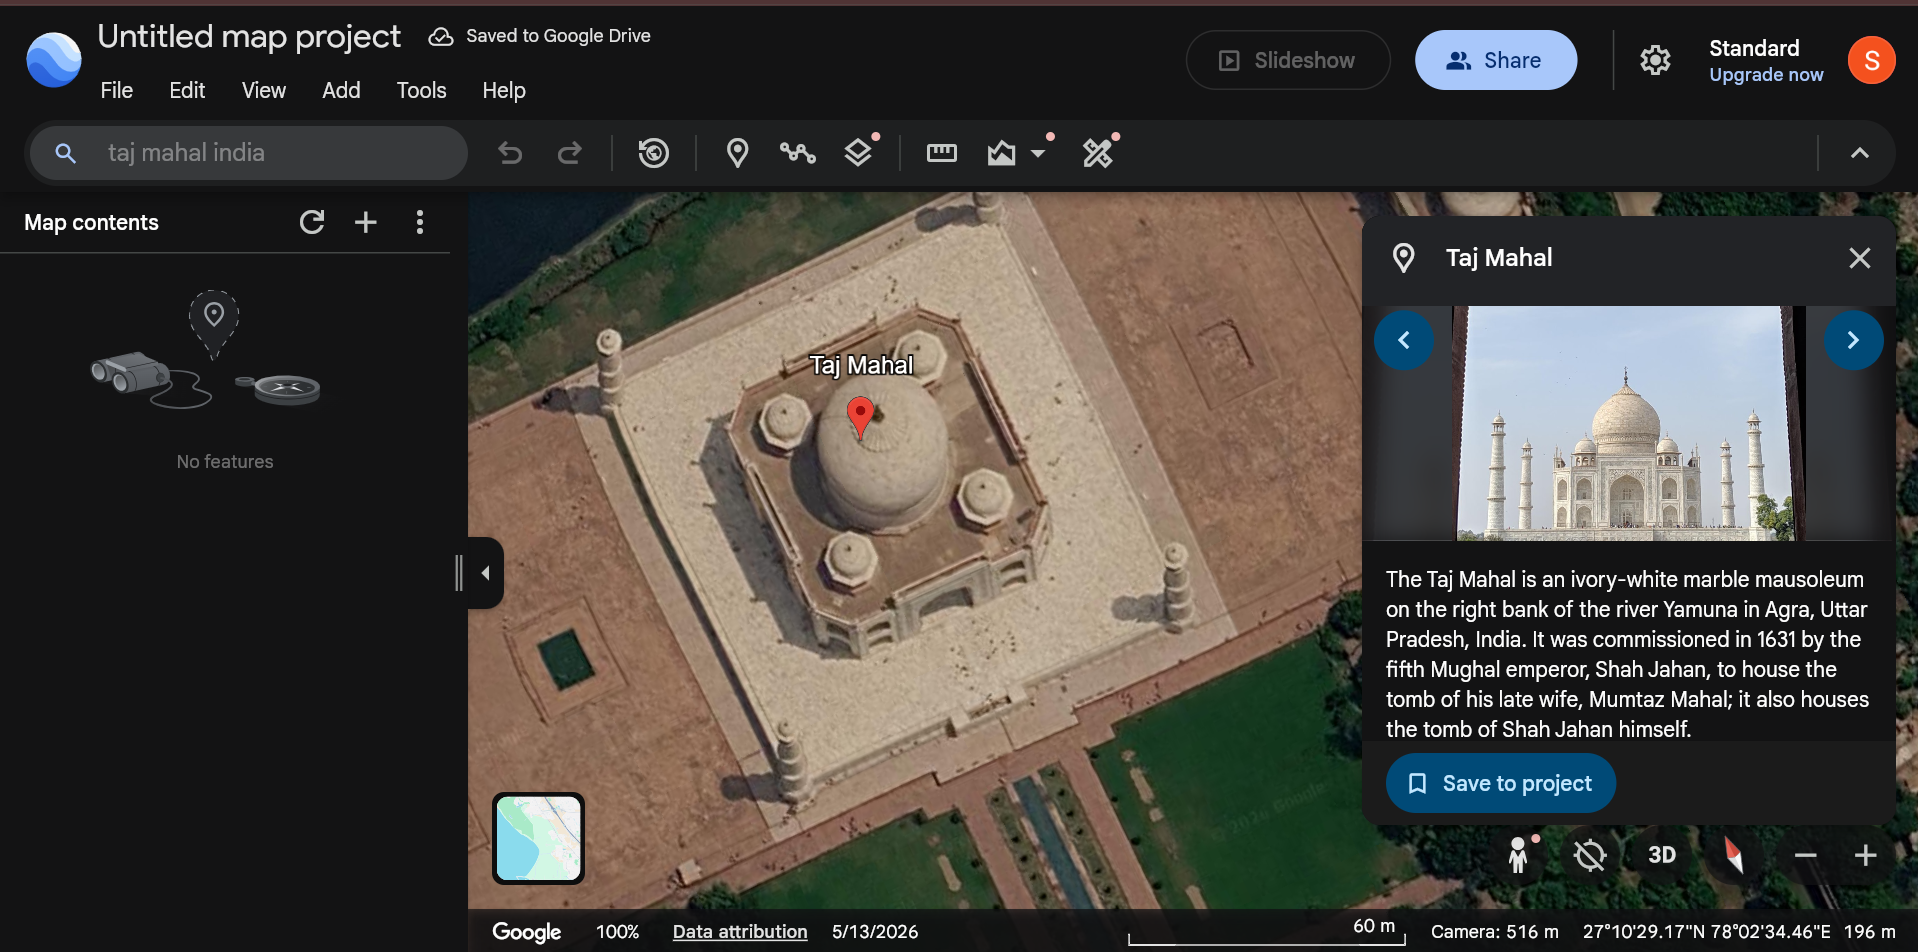
\includegraphics[
        width=18.7cm
    ]{cg_taj_mahal.png}
};


% ============================================================
% CG ANNOTATION 1 -- 3D MESH GEOMETRY
% ============================================================

\node[
    circle,
    fill=Red,
    draw=White,
    line width=1.2pt,
    minimum size=0.60cm,
    inner sep=0pt,
    text=White,
    font=\bfseries\large
]
at ([xshift=8.0cm,yshift=-1.15cm]cg.north west)
{1};

\draw[
    -{Latex[length=3mm]},
    line width=1.5pt,
    Red
]
([xshift=8.0cm,yshift=-1.45cm]cg.north west)
--
([xshift=8.15cm,yshift=-3.25cm]cg.north west);


% ============================================================
% CG ANNOTATION 2 -- TEXTURE MAPPING
% ============================================================

\node[
    circle,
    fill=Red,
    draw=White,
    line width=1.2pt,
    minimum size=0.60cm,
    inner sep=0pt,
    text=White,
    font=\bfseries\large
]
at ([xshift=3.0cm,yshift=-7.25cm]cg.north west)
{2};

\draw[
    -{Latex[length=3mm]},
    line width=1.5pt,
    Red
]
([xshift=3.25cm,yshift=-7.05cm]cg.north west)
--
([xshift=4.85cm,yshift=-6.40cm]cg.north west);


% ============================================================
% CG ANNOTATION 3 -- PERSPECTIVE & DEPTH
% ============================================================

\node[
    circle,
    fill=Red,
    draw=White,
    line width=1.2pt,
    minimum size=0.60cm,
    inner sep=0pt,
    text=White,
    font=\bfseries\large
]
at ([xshift=16.35cm,yshift=-5.05cm]cg.north west)
{3};

\draw[
    -{Latex[length=3mm]},
    line width=1.5pt,
    Red
]
([xshift=16.05cm,yshift=-5.05cm]cg.north west)
--
([xshift=14.75cm,yshift=-4.70cm]cg.north west);

\end{tikzpicture}

\end{center}


% ============================================================
% CG EXPLANATIONS
% ============================================================

\vspace{0.22cm}

\begin{enumerate}[
    label=\textcolor{Red}{\bfseries\arabic*.},
    leftmargin=0.72cm,
    rightmargin=0.25cm,
    itemsep=3pt,
    topsep=0pt,
    parsep=0pt
]

\item
\textbf{3D Mesh Geometry:}
The Taj Mahal is represented through detailed three-dimensional
architectural geometry. The central dome, surrounding structures,
and minarets create recognizable 3D forms and help represent
the landmark in three-dimensional space.

\item
\textbf{Texture Mapping:}
Detailed satellite imagery provides realistic visual textures
for the Taj Mahal, gardens, pathways, water, and surrounding
environment. These surface details improve the visual realism
and context of the 3D scene.

\item
\textbf{Perspective \& Depth:}
The elevated camera position, perspective, object scale, and
spatial arrangement create depth cues. These visual elements
help users understand the relative position, size, and distance
of objects in the 3D environment.

\end{enumerate}


% ============================================================
% PAGE BREAK
% ============================================================

\newpage


% ============================================================
% PAGE 4 -- REFLECTION QUESTIONS
% ============================================================

\pagetitle{REFLECTION QUESTIONS}


% ============================================================
% QUESTION 1
% ============================================================

\begin{center}

\setlength{\fboxsep}{8pt}

\fcolorbox{BorderGray}{LightGray}{%
\begin{minipage}{0.965\textwidth}

\textbf{\color{DarkBlue}
Question 1:
How does the Computer Graphics quality (e.g., realistic
lighting or 3D view) help or hinder the user's ability to
interact with the software?
}

\vspace{0.12cm}

\justifying

The high-quality computer graphics in Google Earth, including
detailed 3D geometry, realistic textures, perspective, and
depth cues, significantly enhance the user's ability to
navigate and understand spatial relationships. The visual
realism makes it easier to recognize landmarks and orient
oneself within the 3D space, which directly supports effective
interaction. However, rendering complex graphics requires
substantial processing power, which can cause performance
issues on older or less powerful devices and may hinder
smooth interaction.

\end{minipage}%
}

\end{center}


% ============================================================
% QUESTION 2
% ============================================================

\vspace{0.22cm}

\begin{center}

\setlength{\fboxsep}{8pt}

\fcolorbox{BorderGray}{LightGray}{%
\begin{minipage}{0.965\textwidth}

\textbf{\color{DarkBlue}
Question 2:
What is one simple HCI change you would make to improve
the user interface?
}

\vspace{0.12cm}

\justifying

One simple HCI improvement would be to add a customizable
``Quick Actions'' toolbar that allows users to pin their most
frequently used tools. Important functions such as measuring
distance, switching to Street View, and changing 3D viewing
options can require users to navigate through menus. A pinned
toolbar would make frequently used tools accessible with a
single click, reducing interaction cost and improving overall
efficiency.

\end{minipage}%
}

\end{center}


% ============================================================
% GRADING BREAKDOWN
% ============================================================

\vspace{0.22cm}

\begin{center}

{\color{DarkBlue}
\fontsize{15}{18}\selectfont
\bfseries
Grading Breakdown
}

\vspace{0.10cm}

\renewcommand{\arraystretch}{1.25}

\begin{tabular}{
    |>{\raggedright\arraybackslash}p{4.0cm}
    |>{\raggedright\arraybackslash}p{16.8cm}
    |>{\centering\arraybackslash}p{1.6cm}|
}

\hline

\rowcolor{DarkBlue}

\textcolor{White}{\bfseries Component}
&
\textcolor{White}{\bfseries Requirement}
&
\textcolor{White}{\bfseries Points}
\\

\hline

\textbf{HCI Annotation}
&
Correctly identifies 3 interaction/UI elements and
their usability purpose.
&
\textbf{35}
\\

\hline

\textbf{CG Annotation}
&
Correctly identifies 3 graphics/rendering elements
such as geometry, texture, perspective, lighting,
or depth.
&
\textbf{35}
\\

\hline

\textbf{Reflection}
&
Clear and concise answers connecting computer graphics
and rendering to the user experience.
&
\textbf{20}
\\

\hline

\textbf{Clarity \& Layout}
&
Clean screenshot layout with easily readable callouts
and pointers.
&
\textbf{10}
\\

\hline

\multicolumn{2}{|r|}{\textbf{TOTAL}}
&
\textbf{100}
\\

\hline

\end{tabular}

\end{center}


% ============================================================
% END OF DOCUMENT
% ============================================================

\end{document}